\section{Inference}
We now focus on the inference dataset (\emph{cyberlab.csv}). First, we applied the same preprocessing adopted previously, truncating words longer than 30 characters. Then, we used the best model identified in \cref{sec:task3} (i.e., UnixCoder-base, $lr=10^{-5}$, 15 epochs) to predict MITRE tags for all the inference sessions, assigning to each bash word the tag associated with the first corresponding token.

\subsection{Predicted tags analysis}
\paragraph{Tags frequency for \texttt{cat}, \texttt{grep}, \texttt{echo}, and \texttt{rm}} \Cref{tab:task4_tags_frequency} summarizes the tag frequencies for the required commands (\texttt{cat}, \texttt{grep}, \texttt{echo}, and \texttt{rm}), computed as the number of times that tag was assigned to a command, divided by the total number of occurrences of that command. Only \texttt{grep} is uniquely associated with a single tag (\emph{Discovery}), while \texttt{cat} is assigned to two different tags: \emph{Discovery} (\SI{90.9}{\percent} of times) and \emph{Execution} (\SI{9.1}{\percent}). \texttt{echo} is mainly associated with three different tags: \emph{Persistence}, \emph{Discovery} and \emph{Execution}. Finally, \texttt{rm} can be assigned to four tags (\emph{Discovery}, \emph{Execution}, \emph{Defense Evasion} or \emph{Persistence}). Some tags are never (or almost) associated with any session; this is the case of \emph{Impact}, \emph{Not Malicious Yet}, and \emph{Other}.

\begin{table}
\small
\centering
\caption{Tags frequency for \texttt{cat}, \texttt{grep}, \texttt{echo}, and \texttt{rm}.}
\label{tab:task4_tags_frequency}
\begin{tabular}{lcccc}
\toprule
{\textbf{Tag}} & {\texttt{cat}} & {\texttt{grep}} & {\texttt{echo}} & {\texttt{rm}} \\
\midrule
Defense Evasion 	& 0.000 	& 0.000 	& 0.000 	& 0.049  \\
Discovery 			& 0.909 	& 1.000 	& 0.334 	& 0.738	\\
Execution 			& 0.091 	& 0.000 	& 0.234 	& 0.196 \\
Impact 				& 0.000 	& 0.000 	& 0.000 	& 0.000 	\\
Not Malicious Yet 	& 0.000 	& 0.000 	& 0.001 	& 0.000 \\
Other 				& 0.000 	& 0.000 	& 0.004 	& 0.000 \\
Persistence 		& 0.000 	& 0.000 	& 0.427 	& 0.017 \\
\bottomrule
\end{tabular}
\end{table}

\paragraph{Session examples} We will now qualitatively analyze one example of a session for each unique tuple (command, predicted tag), focusing only on those appeared more than \SI{1}{\percent} of times.

\textbf{(\texttt{cat}, Discovery):} \texttt{[\dots]; cat /proc/mounts; [\dots]}. This command reads and displays the contents of the file \texttt{/proc/mounts}, listing information about storage devices, network mounts and virtual filesystems. Attackers can use it to map the target system's filesystem structure before attempting further exploitation or lateral movement. Since it's purely information gathering, the tag \emph{Discovery} is appropriate.

\textbf{(\texttt{cat}, Execution):} \texttt{[\dots]; echo
``1'' > /var/tmp/.sysc436621
; cat /var/tmp/.sysc436621 ; [\dots]}\footnote{The file path has been shortened for visualization purposes. The original one is \texttt{/var/tmp/.systemcache436621}.}. In this case, \texttt{cat} reads a hidden file from the temporary directory, created by a previous \texttt{echo}. Even if the \texttt{cat} command itself does not execute any malicious code (it looks like a validation step), it has likely been marked as \emph{Execution} because it precedes the subsequent code execution in the attack chain.

\textbf{(\texttt{grep}, Discovery):} \texttt{cat /proc/cpuinfo | grep name | wc -l ; [\dots]}. The \texttt{grep} command filters the \texttt{cat} output to find lines containing ``name'', enabling the attacker to profile the target system's CPU specifications. The \emph{Discovery} tag looks accurate, since attackers are gathering hardware details before attempting exploitation or lateral movement.

\textbf{(\texttt{echo}, Persistence):} \texttt{[\dots]; echo ``root:XP3IUReH9hhH'' | chpasswd | bash ; [\dots]}. The \texttt{echo} outputs the string \texttt{root:XP3IUReH9hhH} (username:password hash), which is piped to \texttt{chpasswd}, that updates user passwords from standard input. By changing the \texttt{root} user's password to a known value, the attacker gains persistent administrative access to the compromised system.

\textbf{(\texttt{echo}, Discovery):} \texttt{[\dots]; echo ``root 1ntr4n3t'' > /tmp/up.txt ; [\dots]}. It looks like the \texttt{echo} command saves credentials to the \texttt{/tmp/up.txt} file, potentially for future access. Hence, a \emph{Persistence} tag may look more appropriate.

\textbf{(\texttt{echo}, Execution):} \texttt{[\dots]; echo
``base64\_payload'' | base64 --decode | bash ;}. The \texttt{echo} outputs a base64 payload, that is then decoded and executed. Hence, the command immediately executes arbitrary code, not just setting up mechanisms for future access.

\textbf{(\texttt{rm}, Discovery):} \texttt{[\dots]; echo ``321'' > /var/tmp/.v03522123; rm -rf /var/tmp/.v03522123; [\dots]}\footnote{The file path has been shortened for visualization purposes. The original one is \texttt{/var/tmp/.var03522123}.}. This command sequence writes \texttt{321} into the file, and immediately after deletes the same file. Here, \texttt{rm} should probably be marked as \emph{Execution}, since it is an active operation. However, the model may have marked it as \emph{Discovery} as it is surrounded by file operations that can be associated with a discovery phase, for example as a permission check.

\textbf{(\texttt{rm}, Execution):} \texttt{[\dots]; rm -rf /var/tmp/dota* ; [\dots]}. This command deletes the files in the directory \texttt{var/tmp/dota}. Hence, it is active operation, removing files that may contain traces of previous actions. However, in that case the \emph{Defense Evasion} tag would be more appropriated.

\textbf{(\texttt{rm}, Defense Evasion):} \texttt{[\dots]; cp /bin/echo .s ; [\dots]; rm .s ; exit}. This command sequence copies the \texttt{echo} binary in \texttt{.s}, that is finally deleted as last step. This operation is clearly \emph{Defense Evasion} because it's the final cleanup step that removes forensic evidence of the attack.

\textbf{(\texttt{rm}, Persistence):} \texttt{[\dots]; echo ``admin Passwd4'' > /tmp/up.txt ; rm -rf /var/tmp/dota*}. This command deletes the files in the directory \texttt{var/tmp/dota}. Hence, it looks like \emph{Defense Evasion} technique, removing files that may contain traces of previous actions. However, the model probably consider it as \emph{Persistence} due to the previous steps, such as the \texttt{echo} command that saves the credentials to the \texttt{/tmp/up.txt} file, making them persistent across restarts.


\subsection{Fingerprint Analysis}
Subsequently, we focused on the fingerprints present in the inference dataset. After having identified the unique fingerprints, we sorted them by ``date of birth'' and we assigned to each an ID. Then, we counted the number of sessions described by a specific fingerprint for each date.

\Cref{fig:fingerprintTimeline} shows fingerprints IDs appearance over time: the y-axis lists fingerprint IDs (the lower the value, the earlier the fingerprint appeared for the first time), while the x-axis represents the full data-collection period. Each point indicates that at least one session associated with that fingerprint occurred on that date. The size and color of each point reflect how many sessions for that fingerprint were recorded that day: larger and redder points correspond to more sessions.

\paragraph{Fingerprint patterns}  The plot reveals clear temporal and structural patterns in the inference dataset. During the collection period, 15516 unique fingerprints were observed: horizontal bands indicate fingerprints that reappear over multiple days or weeks, while vertical columns refer to daily batches of observed fingerprints. In the first one month and a half, a relatively small number of unique fingerprints appeared ($\approx1150$), while by 1st December this number increased significantly, reaching $7000$. In the final month, more $7000$ new fingerprints appeared, and the vertical columns became denser (excluding a day in mid-December, in which no session is received). However, in the last week of collection, many fingerprints disappeared or became rare, as shown by the sparse points. The last appeared (those with ID $\approx15000$) continued arriving.

\paragraph{Most present fingerprints} A subset of fingerprints, primarily with low IDs ($<500$), appears persistently throughout the entire observation period with relatively stable and low session counts. In particular, the fingerprints present on most days are those with IDs 0, 17, 19 and 21 (99 days of presence over 122). However, some of them stopped appearing or became rarer in the last period of collection (from 10th December).

\paragraph{Fingerprints with more sessions} Some fingerprints have many associated sessions: examples are fingerprint 21 (26036 sessions), 48 (17639), 25 (7169), 42 (4479) and 8858 (4342). However, these numbers do not always translate in red big circles on the plot, since many sessions span across the whole collection period: the medium-sized yellow/orange clusters at the bottom indicate ``regular'' fingerprints.

\paragraph{Attack campaigns} Several fingerprints exhibit burst-like behavior, characterized by sudden appearance and high numbers of associated sessions over short time intervals. Most notably, a dominant fingerprint (8858) emerging in mid-December 2019 (8th-10th) reaches the highest session count per day ($>1000$) in the dataset, strongly indicating a coordinated attack campaign. This fingerprint is initially characterized by a \emph{Discovery} phase, followed by some \emph{Persistence} action. Then, there are many \emph{Discovery} commands, some \emph{Execution} actions, and finally \emph{Persistence} steps. Hence, after an exploratory phase, the attacker is probably executing an exploit, finally making its impact persistent. Additionally, the late-December period shows a dense concentration of high-ID fingerprints with moderate to high activity, consistent with a possible attack campaign.

\begin{figure}
	\centering
	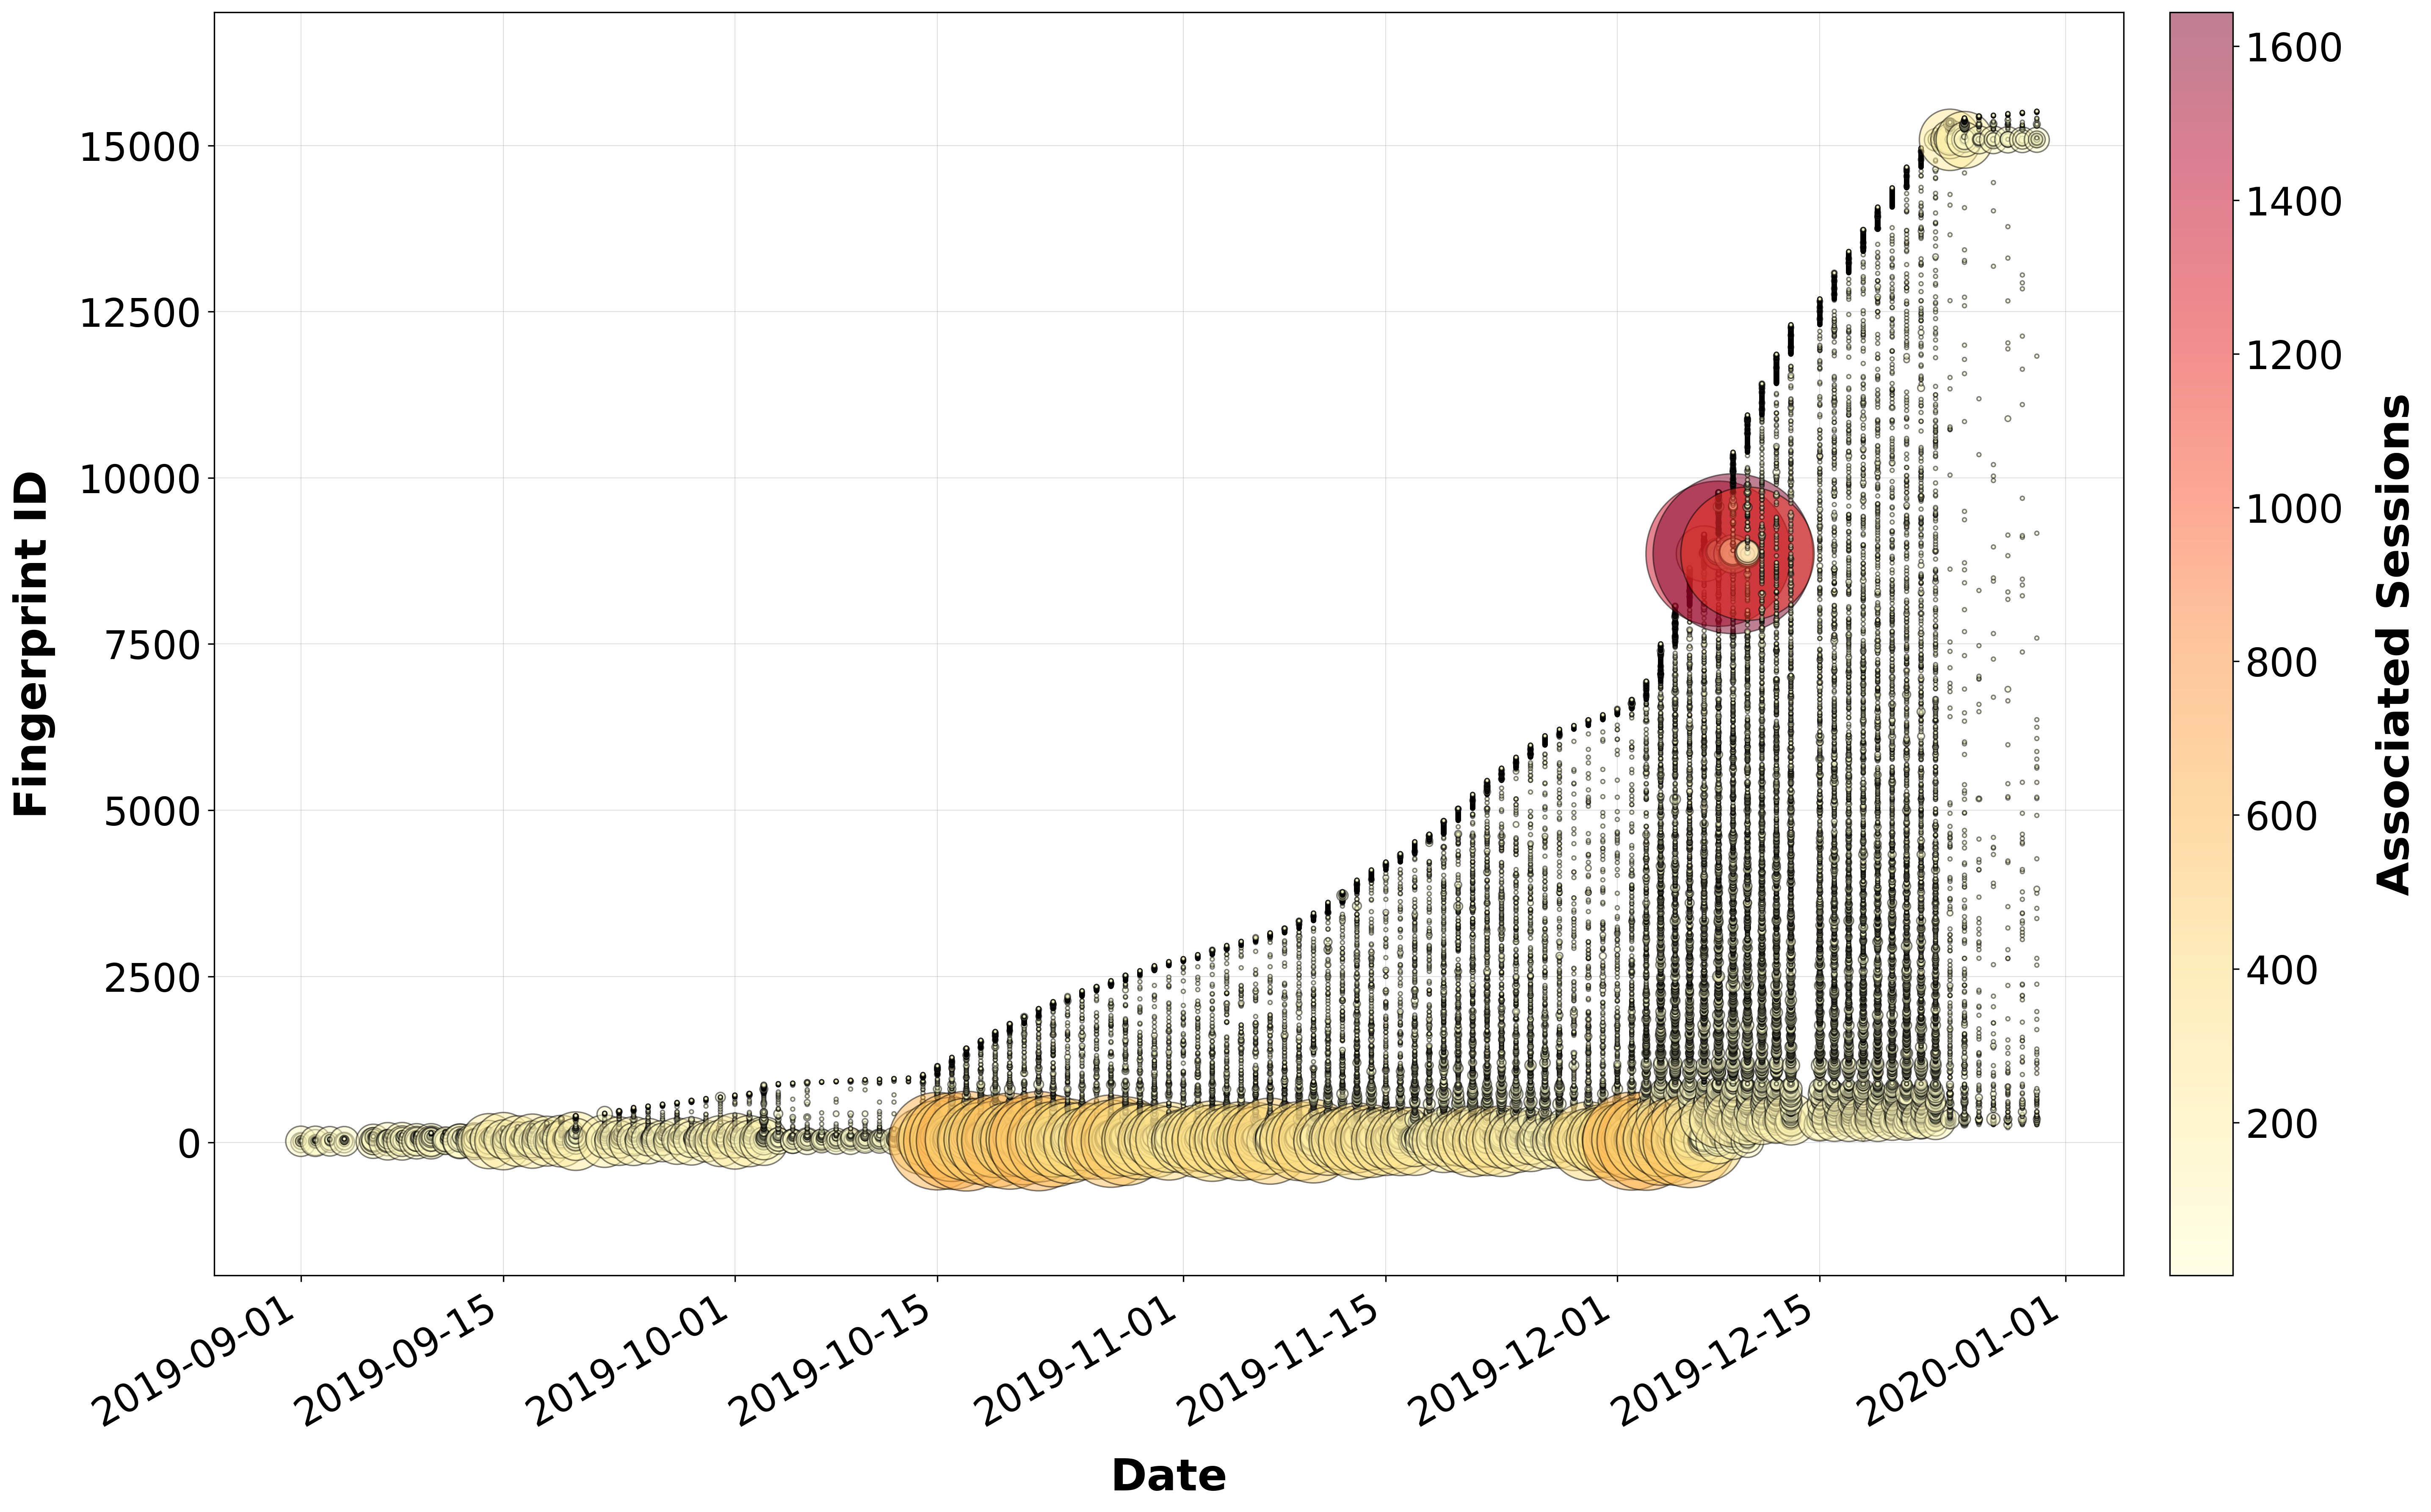
\includegraphics[width=0.9\linewidth]{img/Task4/fingerprint_timeline_small_circles.png}
	\caption{\textbf{Fingerprint IDs over time.} The y-axis lists fingerprint IDs, ordered by when they were first observed in the honeypot – the earliest-seen fingerprints
appear at the bottom. The x-axis represents the full data-collection period. Each point indicates that at least one session associated with that fingerprint occurred on that date. The size of each point reflects how many sessions for that fingerprint were recorded that day: larger points correspond to more sessions.}
	\label{fig:fingerprintTimeline}
\end{figure}